%\documentclass[a4paper,11pt]{scrreprt}
%\documentclass[a4paper,15pt]{scrbook}
\documentclass[a4paper,12pt]{scrartcl}
%\documentclass[a4paper,13pt]{scrreprt}

\usepackage[T1]{fontenc}
\usepackage[utf8]{inputenc}
%\usepackage[latin9]{inputenc}
\usepackage{scrpage2}
\usepackage{titleref}
\usepackage[ngerman]{babel}
\usepackage{multicol}
\usepackage{lmodern}  
\usepackage{tabularx} 
\usepackage{graphicx}
\usepackage{blindtext}
\usepackage{microtype}
\usepackage{color}
\usepackage{colortbl}
\usepackage{framed} %umramen eines Bereiches
%\usepackage[left=25mm,right=25mm,top=25mm,bottom=25mm]{geometry} % Standard
%\usepackage[left=20mm,right=20mm,top=25mm,bottom=30mm]{geometry}
%\usepackage[singlespacing]{setspace}
\usepackage[onehalfspacing]{setspace}
%\usepackage[doublespacing]{setspace}
\usepackage{verbatim}
\usepackage{listings}
%\usepackage[svgnames]{xcolor}
\usepackage{xcolor} 
\usepackage{setspace}
\usepackage{amsthm}
\usepackage{float}
\usepackage{pdfpages}
\usepackage{mdwlist}
\usepackage{prettyref}
\usepackage{multicol}
\usepackage[section]{minted}	
\usepackage{hyperref}

%%%%%% Beschriftung
\newcommand{\changefont}[3]{
\fontfamily{#1}\fontseries{#2}\fontshape{#3}\selectfont}


%\include{./color}
%\include{./environment}
%\input{./minted}
%\input{./listings}	
	
\begin{document}
%-------------------------------------
% Titelseite 
\thispagestyle{empty}
\begin{center}
	
\includegraphics[scale=.5]{./fau}\\
	\vspace*{2cm}
	\Large
	\textbf{Informatik}\\
	\textbf{Marketing Fallstudien}\\
	\vspace*{2cm}
	\Huge
	\textbf{Hausarbeit}\\
	\vspace*{0.5cm}
	\large
	über das Thema\\
	\vspace*{1cm}
	\textbf{Neue Gefahren durch neue Apps und Foren wie YouNow und Snapchat}\\
	\vspace*{2cm}
	
	\vfill
	\normalsize
	\newcolumntype{x}[1]{>{\raggedleft\arraybackslash\hspace{0pt}}p{#1}}
	\begin{tabular}{x{6cm}p{7.5cm}}
		\rule{0mm}{5ex}\textbf{Autor:} & Johannes Pfann \newline johannes.pfann@fau.de \\
		\rule{0mm}{5ex}\textbf{Autor:} & Johannes Stadlinger \newline johannes.stadlinger@fau.de \\
		\rule{0mm}{5ex}\textbf{Abgabedatum:} & \today \\
	\end{tabular} 
\end{center}
\pagebreak

%-------------------------------------

%-------------------------------------
% Verzeichnisse  
\tableofcontents % Inhaltsverzeichnis
\pagebreak
%\listoffigures % Abbildungsverzeichnis 
%\listoftables % Tabellenverzeichnis 
%-------------------------------------

%-------------------------------------
% Textkörper
%%%%%%%%%%%%%%%%%%%%%[Einleitung]
\section{Zusammenfassung}
Das Thema soziale Netzwerke wurde in den letzten Jahren immer populärer. In den letzten 5 Jahren hat sich die Anzahl mehr als verdoppelt. Vor allem durch Mobile Anwendungen hat sich die Benutzung dieser soziale Netzwerke dramatisch verändert. Problematisch ist dabei, das Jugendliche sich der Konsequenz dieser Veränderung nicht bewusst sind.
Die folgende Hausarbeit beschäftigt sich mit Gefahren durch die Apps und Foren wie YouNow und Snapchat im Rahmen der Veranstaltung Marketing Fallstudie. Ziel dieser Arbeit ist ein grundsätzliches Verständnis der Anwendungen YouNow und Snap-Chat zu beschreiben um dann die Gefahren durch Pädophilie und Datenschutzrecht zu erläutern.
 


\section{Einleitung}
Das Thema \emph{soziale Netzwerke} wurde in den letzten Jahren immer
popul\"arer. Wie man in Abbildung~\ref{fig:overall} sieht, waren es im Jahr
2010 lediglich knapp eine Milliarde Nutzer weltweit, die sich in solchen
Netzwerken angemeldet hatten. Die Zahl stieg stetig an. Innerhalb von f\"unf
Jahren (2015) hat sich diese Anzahl mehr als verdoppelt auf $2,14$ Milliarden
Nutzer. Das stetige Wachstum wird auch f\"ur die Zukunft prognostiziert.
\begin{figure}[ht]
	\centering
	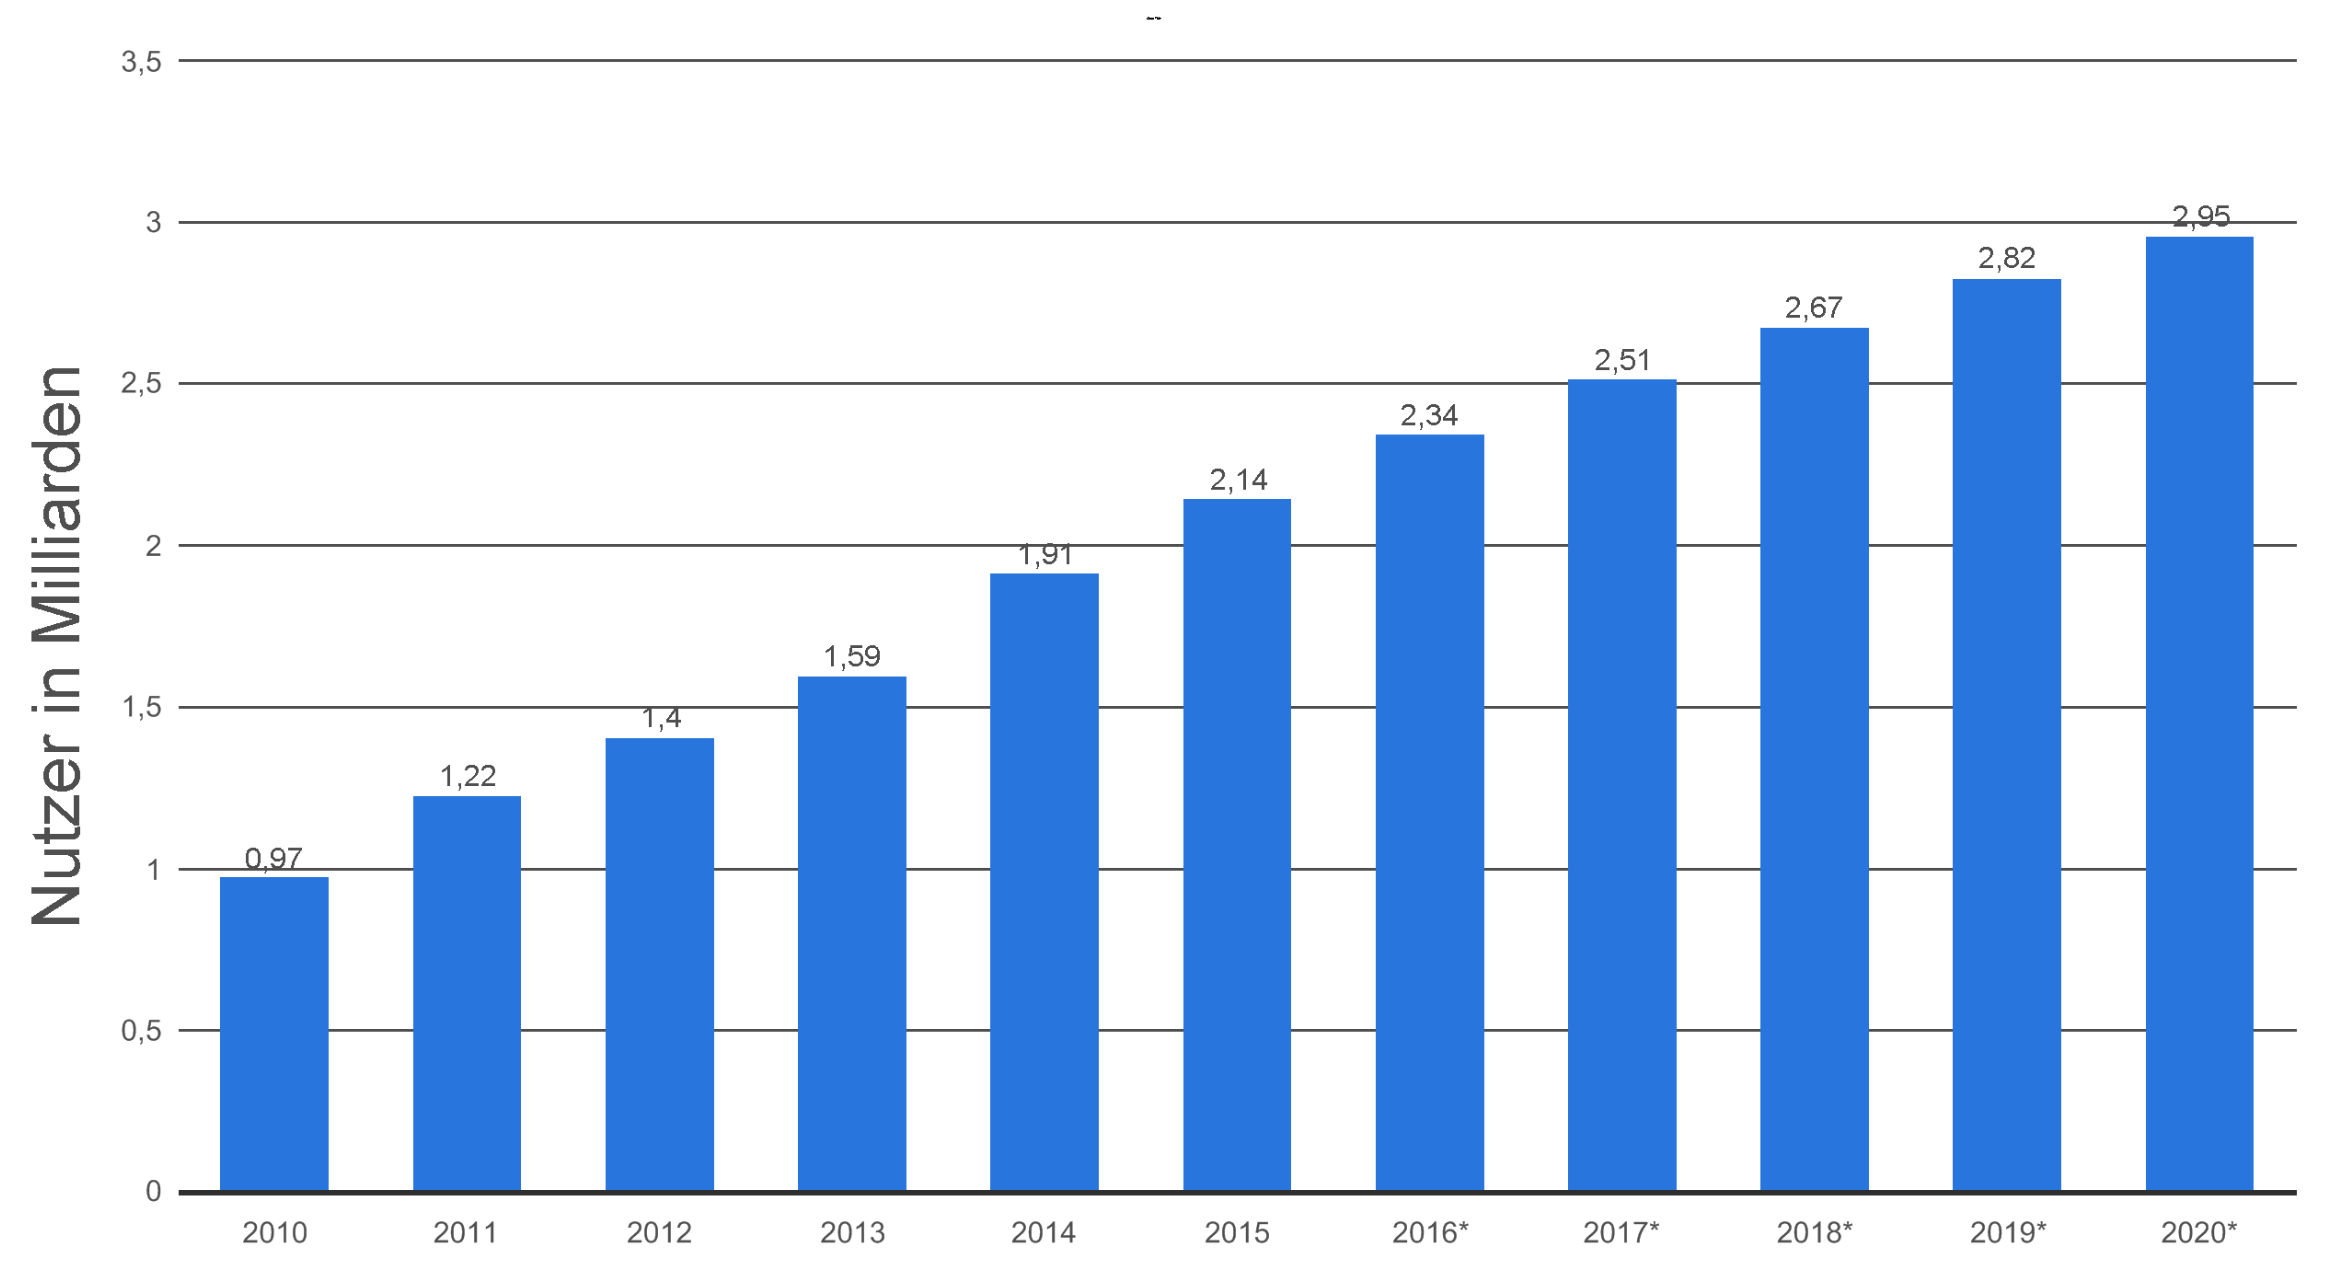
\includegraphics[scale=0.6]{resources/einf_02.png}
	\caption{Anzahl der Nutzer sozialer Netzwerke weltweit in den Jahren 2010
	bis 2015 sowie eine Prognose bis 2020 (in Milliarden)~\cite{statista-allg}.}
	\label{fig:overall}
\end{figure}

//hier noch etwas text. Uebergang von allg. zu Jugendlichen. evtl noch mehr statistiks

YouNow\footnote{\url{https://www.younow.com}} und
SnapChat\footnote{\url{https://www.snapchat.com}} sind zwei aufstrebende,
neuere Anwendungen in diesem Bereich und vor allem bei Kindern und Jugendlichen
sehr beliebt~\cite{statista-snapchat, vaterlaus2016snapchat}. Im Rahmen dieser Arbeit werden beide
etwas n\"aher betrachtet und auf m\"ogliche Gefahren in Bezug auf P\"adophilie
untersucht.


\section{YouNow}
\subsection{Beschreibung}
YouNow ist eine kostenlose Live-Videostreaming-Plattform, die als App auf dem Smartphone oder als Desktop-Anwendung verfügbar ist. Nutzer können nach einer Anmeldung mit der Kamera ihres Smartphones, Laptop oder Tablets Live-Streams von sich aufnehmen und für andere Nutzer bereitstellen oder bei dessen Live-Streams zusehen. Neben der Möglichkeit des Live-Streams bietet die Plattform einen Chat an, sodass in einem Live-Stream alle Beteiligten miteinander kommunizieren können. Außerdem kann ein weiterer Nutzer sich an einem Video beteiligen. 

\paragraph{Anmeldung}
Nach Installation der App auf dem Smartphone oder dem Öffnen der Website mit dem Browser kann man sich mit Facebook, Gmail- oder Twitter-Account anmelden. Diese Anmeldung erfordert allerdings sämtliche Kontaktdaten und Email-Adressen des Kontoinhabers. Außerdem muss man versichern, das man nicht jünger als 13 Jahre alt ist.
Im nächsten Schritt wird man aufgefordert einen Namen anzugeben, mit dem man in Videos und Chats erkannt wird.

\paragraph{Kommunikation}
Während des Live-Streams ist gleichzeitig ein Chat aktiv, mit dem sich der Protagonist mit seinen Zuschauern unterhalten kann. Chatteilnehmer können sich Nachrichten, Sticker oder Icons zusenden. Neben den Chats, ermöglicht die App das Versenden von Posts zu einzelnen Personen. Diese erscheinen, ähnlich wie bei der Facebook-Chronik, auf einer Pinnwand der jeweiligen Person. Außerdem können sich YouNow-Nutzer private Nachrichten zusenden.


\paragraph{Geschenke und Währung}
Bei YouNow gibt es zwei verschiedene Währungen die jeweils für verschiedene Aktionen gedacht sind. Zum einen gibt es Münzen (Coints), die repräsentieren einen Wert eines Geschenkes. Mit einem Geschenk, kann ein Zuschauer auf sich aufmerksam machen bzw. den Stream eines anderen wertschätzen, indem er ein Geschenk für diesen versendet. Geschenke sind in diesem Fall kleine Bilder (Icons).
Coints haben keinen realen Gegenwert und müssen in YouNow verdient werden. Mit folgenden Aktionen können Coints verdient werden:

\begin{itemize}
	\item Veröffentlichen von Livestreams
	\item Aktive Teilnahme. Durch das Anschauen von Livestreams, Liken oder chatten kann man Münzen verdienen.
	\item Deine Freunde für eine Anmeldung bei YouNow werben. Für jede Anmeldung deiner Freunde über einen Facebook-Post, Tweet, E-Mail, Tumblr-Verlinkung oder Facebook-Einladung von dir erhältst Du Münzen. 
	\item Dich jeden Tag anmelden.
\end{itemize} 

Eine weitere Währung sind die sog. \textbf{bars}. Diese können nicht durch Aktionen erworben werden, sondern müssen gekauft werden. Die haben also einen realen Gegenwert. Mit diesen können dann Premiumgeschenke gekauft werden, mit denen man sich in einem Chat besonders auf sich aufmerksam machen kann. Premiumgeschenke könnten sein:

\begin{itemize}
	\item 50 Likes: Ein Geschenk, dass den Broadcaster hilft zu trenden
	\item Fanpost: Eine personalisierte Chat-Nachricht, die heraussticht 
	\item 50 Likes für den eigenen Stream: Hilft dem Broadcaster, mehr Aufmerksamkeit zu erlangen
	\item Chat-cool-down-bypass: Aufhebung der Begrenzung der eigenen Chatnachrichten in vollen, überlasteten Chats
	\item Bars: Um Partner unmittelbar zu unterstützen
\end{itemize}

\paragraph{Levelsystem}
YouNow führt außerdem ein Levelsystem ein. Dieses hat die Aufgabe den Nutzer dazu anzuregen mehr Aktionen auf YouNow zu tätigen. Der Anreiz um weitere Levels zu bekommen ist, dass der Nutzer dadurch Zugriff auf bessere und speziellere Geschenke erlangt um den Streamenden zu unterstützen. Außerdem steigt pro Level auch der Wert an Münzen, die dann auf die normalen Geschenke berechnet werden. 
Um ein höheres Level zu erreichen hat der Nutzer folgende Möglichkeiten.

\begin{itemize}
	\item je mehr Geschenke sie selbst erhalten
	\item je mehr Likes sie erhalten
	\item je größer ihr Publikum ist
	\item je mehr Live-Streams sie tätigen
	\item je mehr sie mit anderen Nutzern chatten
	\item je mehr Geschenke sie selbst vergeben
	\item je mehr Freunde sie zu YouNow einladen.
	\item und, wenn sie ihre Konten aus anderen Sozialen Netzwerken, wie z. B. YouTube, Facebook, Twitter mit ihrem YouNow-Konto verknüpfen.
\end{itemize}


\section{Snapchat}
Snapchat ist eine kostenlose Smartphone Anwendung f\"ur Android und iOS, die es
seinen Nutzern erm\"oglicht Bild- sowie Videonachrichten zu versenden. Die App
wurde im September 2011 initial released und ist mittlerweile in $20$ Sprachen
\"ubersetzt. Im Gegensatz zu YouNow gibt es f\"ur Snapchat keine
Desktopvariante.

Eine Besonderheit gegen\"uber anderen Anwendungen ist, dass die Medieninhalte
nur f\"ur begrenzte Zeit, d.h. mindestens eine und maximal $10$ Sekunden
f\"ur den/die Empf\"anger sichtbar sind. Nach diesem Zeitraum l\"oschen sich
laut Anbieter die Dateien von selbst beim Client. Mittlerweile ist es jedoch
m\"oglich die Inhalte mehrfach anzusehen. Zudem kann ein Nutzer eine sogenannte
,,Snapchat-Geschichte'' anlegen, welche $24$ Stunden sichtbar und mit
bestimmten Freunden oder der gesamten Community teilbar ist.

\paragraph{Anmeldung}
Bevor man die Anwendung auf seinen Smartphone installieren kann, muss man
Snapchat umfangreiche Rechte zugestehen. Abbildung~\ref{fig:sc_perms} zeigt
examplarisch die Rechteanfordungen unter Android.
\begin{figure}[ht]
	\centering
	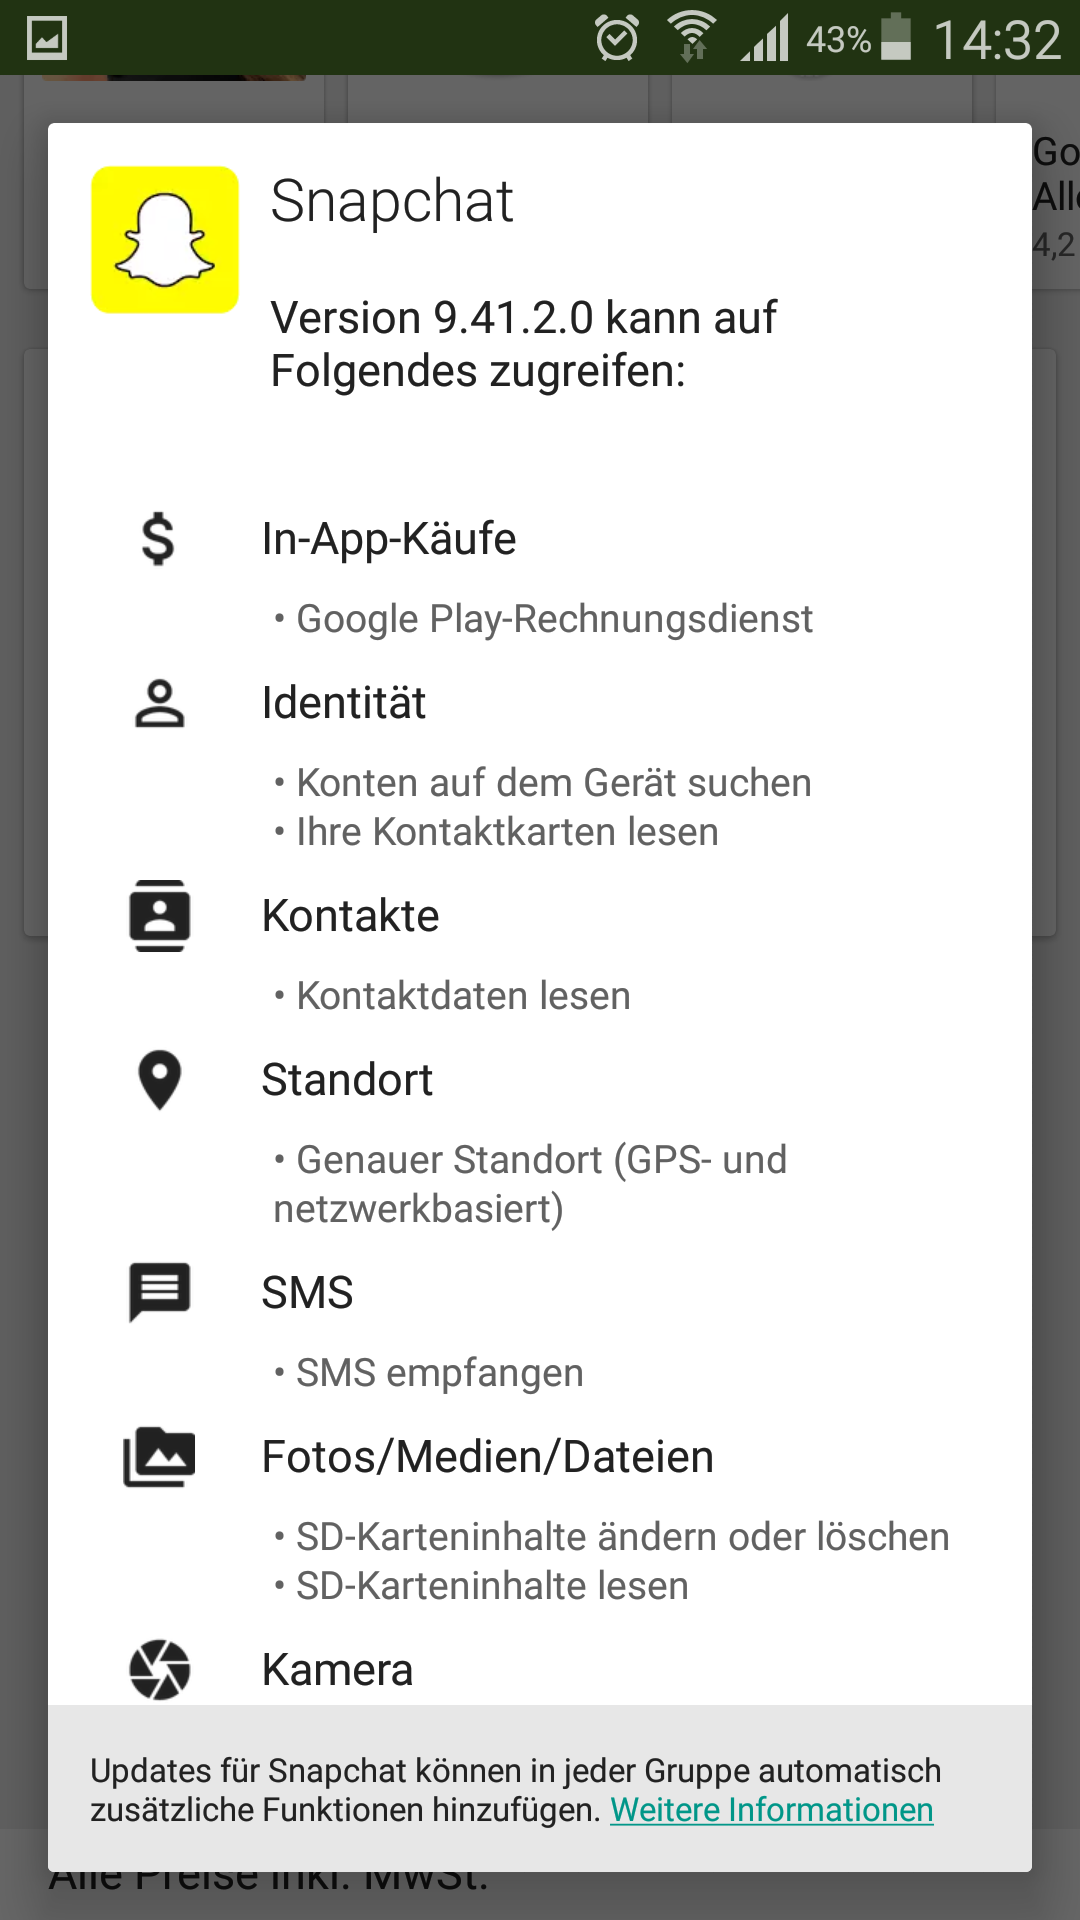
\includegraphics[width=0.4\linewidth]{resources/sc_perms_1.png}
	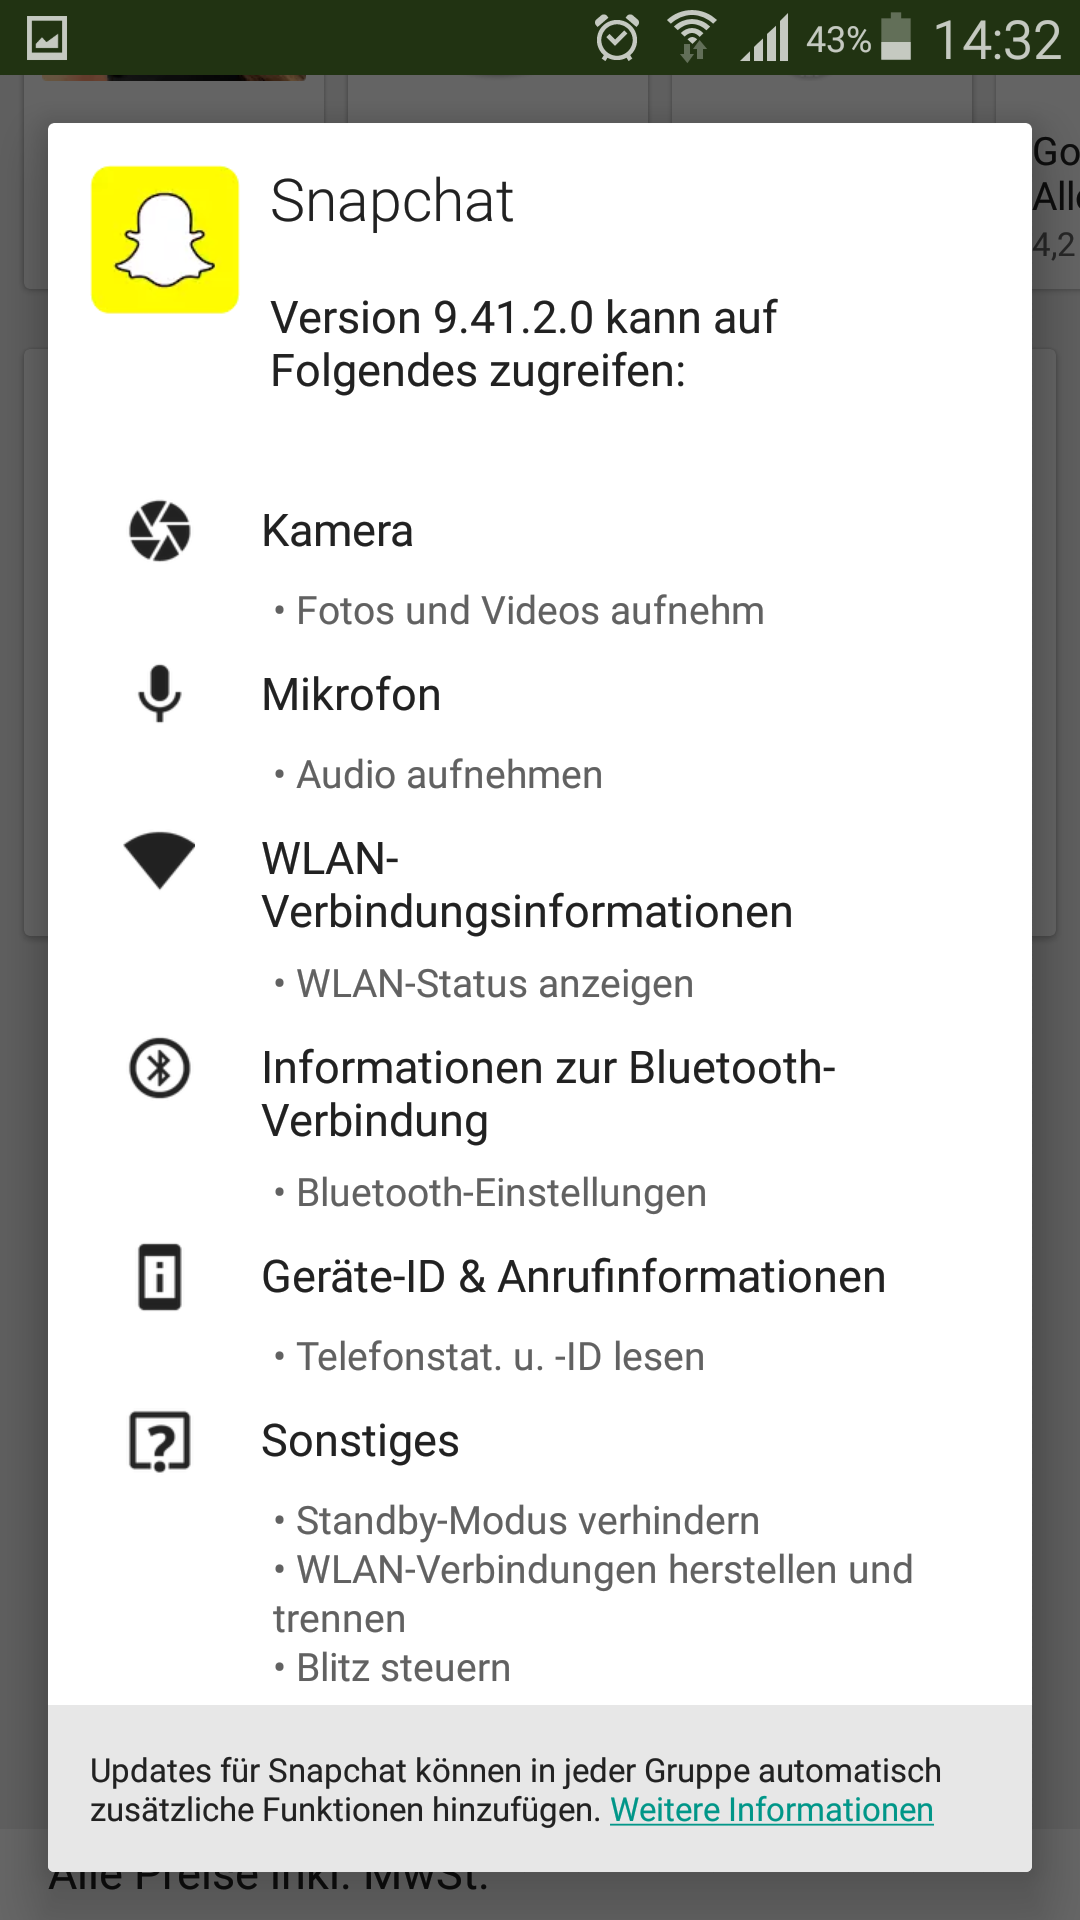
\includegraphics[width=0.4\linewidth]{resources/sc_perms_2.png}
	\label{fig:sc_perms}
	\caption{\"Ubersicht der Rechteanforderung von Snapchat auf einem Android
	Smartphone.}
\end{figure}
Unter anderem muss der App das Auslesen s\"amtlicher Kontakt- sowie
Standortdaten des Ger\"ats gew\"ahrleistet werden. Auch der Zugriff auf
Fotos, Videos, Medien sowie Kamera und Mikrofon muss freigegeben werden.

Ist die App auf dem Ger\"at installiert kann man sich als Nutzer anmelden.
Hierf\"ur ist eine Email-Adresse, ein Nutzername, das Geburtsdatum, sowie ein
Passwort erforderlich. Eine Kontrolle des Alters wird vom Anbieter nicht
durchgefuehrt.

\paragraph{Funktionsweise und Kommunikation}
In diesem Abschnitt m\"ochten wir noch etwas genauer auf die Funktionsweise und
Kommunikation von Snapchat eingehen.

Um \"uberhaupt Inhalte zu Versenden braucht der neu angemeldete Nutzer Personen
mit denen er kommunizieren kann. Diese kann er \"uber folgende M\"oglichkeiten
hinzuf\"ugen:
\begin{itemize}
	\item Nutzernamen: Eingabe konkreter Nutzer.
	\item Aus Kontakten: Kontaktliste des Smartphones nach Personen mit
	Snapchat durchsuchen lassen.
	\item Snapcode: Vergleichbar mit QR-Codes.
	\item In der N\"ahe: Nutzer, die im gleichen Wlan-Netz sind.
\end{itemize}

Jetzt hat der Nutzer die M\"oglichkeit sogenannte \emph{Snaps} d.h. Fotos oder
Videos aufzunehmen bzw. aus der Gallerie zu entnehmen und diese mit Text,
Filtern, etc. zu bearbeiten. Anschliessend kann er diese an seine Freunde
schicken. Wie eingangs erw\"ahnt, kann er nun auch festlegen, wie lange das
Medium auf dem Ger\"at des Empf\"angers sichtbar bleibt (eine bis max. zehn
Sekunden). Nach diesem Zeitraum wird das Datum vom Endger\"at gel\"oscht. Zudem
hat er die M\"oglichkeit das Medium seiner eigenen \emph{Geschichte} (engl.:
\emph{story}) hinzuzuf\"ugen damit es $24$ Stunden sichtbar bleibt. Von dort
aus kann er seine Snaps mit Freunden oder mit der ganzen Community teilen. Die
Inhalte k\"onnen dann von allen Beteiligten gespeichert werden.

Neben der M\"oglichkeit seinen Partnern Text-, Bild- und Snapnachrichten zu
schicken, bietet Snapchat auch einen Videochat an. Hier kann man sich in
Echtzeit mit seinem Gegen\"uber mit Hilfe seiner Smartphonekamera unterhalten.



\pagebreak
%%%%%%%%%%%%%%%%%%%%%[Quellen]
\section{Quellen}
%%%%%%%%%%%%%%%%%%%%%%%%%%%%%%%%%%%%%%%%%%%%%%%%%%%%%%%%%%%%%%%%%%%%%%%%%%%%%%%
%
%  http://www.weinelt.de/latex/thebibliography.html
%  \bibitem[Markierung]{Kennung}Quelle
%  \cite[Spezifikation]{Kennung}
%  \cite{GARR05}) kann auf die Quelle zugegriffen werden
%
%%%%%%%%%%%%%%%%%%%%%%%%%%%%%%%%%%%%%%%%%%%%%%%%%%%%%%%%%%%%%%%%%%%%%%%%%%%%%%%

\begin{thebibliography}{12cm}

\bibitem[GOF95]{GOF95} Erich Gamma, Richard Helm, Ralph E. Johnson, John Vlissides: Entwurfsmuster. Elemente wiederverwendbarer objektorientierter Software. Addison-Wesley, München 2004, ISBN 3-8273-2199-9.

\bibitem[EIST06]{EIST06} Karl Eilebrecht, Gernot Starke: Patterns Kompakt: Entwurfsmuster für effektive Softwareentwicklung Spektrum Akademischer Verlag, 4 Auflage 2006, ISBN 3-8274-1443-1

\bibitem[IN15]{IN15} Michael Inden: Der Weg zum Java-Profi: Konzepte und Techniken für die professionelle Java-Entwicklung, dpunkt.verlag,Heidelberg 2015, ISBN 978-86490-203-1

   

\end{thebibliography}


\end{document}